% \glsresetall
\chapter{State of technology} % Main chapter title
\label{Chapter2}

\lhead{Chapter 2. \emph{State of technology}}

In this chapter the current state of technologies which can provide possible solutions for the issue of redundant resources in a micro frontend landscape is explained. Additionally, an overview about the used Luigi framework is given.

\section{Micro frontend framework Luigi}
\label{mf_framework_luigi}

Currently there are different micro frontend frameworks present on the market. Some of which are \textbf{Bit, SystemJS, Webpack 5 Module Federation, Piral, Single SPA} and \textbf{Luigi}.\cite{top10_mffs}
For the implementation of the representative landscape the Luigi framework was used, therefore a short introduction of it is given here.

\subsection{Luigi}

Luigi is an open source JavaScript framework for micro frontends, consisting of two main parts, the \textbf{Luigi Core} and the \textbf{Luigi Client}. It provides a basis to integrate micro frontends, also called \textbf{Nodes} in this context. Both parts serve different purposes in the micro frontend landscape.\cite{luigi_doc_overview}

\subsubsection{Core}

The \textbf{Luigi Core} is the groundstone of the whole landscape. It defines the main app, which will serve as an entry point for the user. The possible, applicable configurations of this part are the following:

\begin{itemize}[noitemsep]
	\item Navigation
	\item Authorization
	\item Localization - providing translations to display its applications in multiple languages
	\item General settings - e.g. header display configurations, apply loading indicators for the micro frontends, etc.
	\item Luigi Core API - providing functions for the core app to interact with the framework and access its features
\end{itemize} 

The core application inside the landscape is determined via the \texttt{luigi.config.js}. Any project containing it can fulfill this role, which is the only prerequisite. In the context of the framework this app is later referred to as the \textbf{Core}.
Following this principle, the project structure of the \textbf{Core} could look as shown in \ref{luigi_core_structure}.\footnote{This example is directly taken from the implemented core project.}  

\begin{lstlisting}[language=Bash, caption=Project structure for a Luigi Core application including the \texttt{luigi.config.js}, label=luigi_core_structure]
	- react-core-mf
		- [...]
		- node_modules
		- public
			- [...]
			- index.html
			- luigi.config.js
		- [...]
		- src
\end{lstlisting}

In the \texttt{luigi.config.js} itself the above mentioned possible configurations are defined.\cite{luigi_doc_core}

\subsubsection{Client}

The Luigi Client serves as the connection between the framework and its micro frontends. In order to establish the connection a micro frontend has to import and initialize it. This will grant the micro frontend access to the \textbf{LuigiClient} object during the runtime. The micro frontend can then interact with the framework to e.g. set a global state, add event listeners or enable navigation between other micro frontends in the landscape.

An import of the Luigi Client can be accomplished via different methods. The most forward approach, might be the direct import with a HTML script tag. Another option can be the import of the local package manager dependency.\cite{luigi_client}

\begin{lstlisting}[caption=Import methods of the Luigi Client]
	<!-- Via the HTML script tag -->
	<script src="https://unpkg.com/@luigi-project/client@1.17.0/luigi-client.js">
	</script>
	
	<!-- Via the package manager -->
	import LuigiClient from "@luigi-project/client";
\end{lstlisting}

\subsection{Architecture}

After the short introduction of the framework's core components, a general architecture of a landscape implemented with it is provided below.

\begin{figure}[!h]
	\centering
	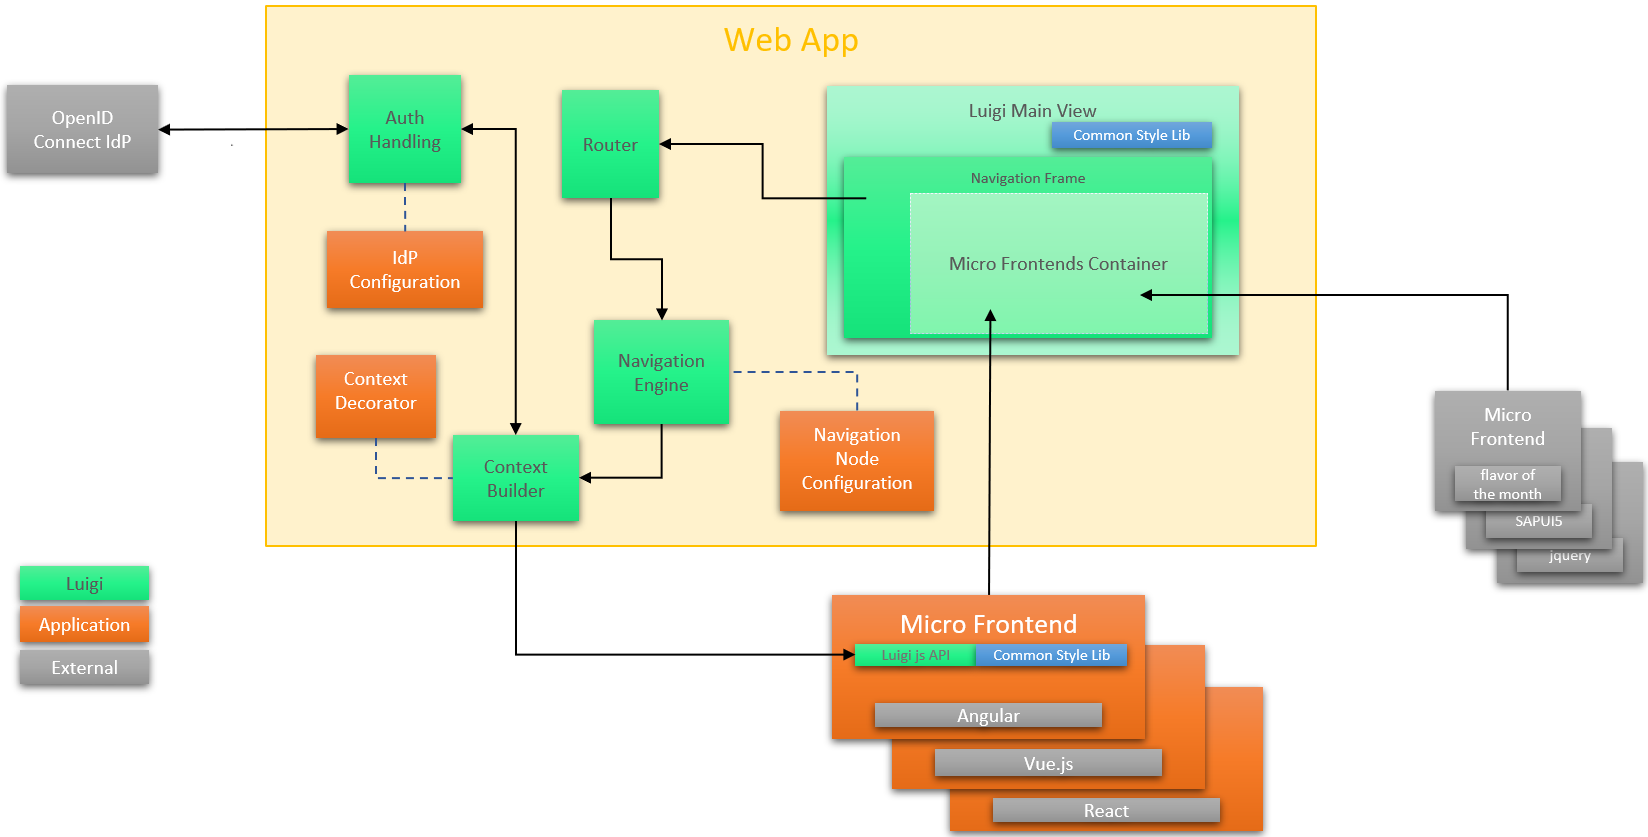
\includegraphics[width=1\textwidth]{Figures/Luigi_Architektur.png}
	\caption{Architecture of the Luigi Framework \cite{luigi_architecture}}
	\label{fig:luigi_architecture_fig}
\end{figure}

As can be seen in figure \ref{fig:luigi_architecture_fig}, the displayed micro frontends in the Web App have a distinguished position in the Micro Frontends Container. The embedded projects can either be integrated via iFrames or as Web Components as so called Compounds.
Via the provided dashboard, called Navigation Frame in the image, the Luigi Core features are used. Through it the navigation or search feature can be accessed.

As described in the first chapter of this transcript, the issue in such a landscape is redundancies between the same libraries of the embedded micro frontends. Each Node is an isolated application, which is the reason for this problem.
For instance, navigating to the first micro frontend and then followed by the second one will load the bundled projects with their corresponding dependencies. In this case the browser has no way to distinguish if a loaded resource is already present or not. Reason for that is the bundling of the projects which makes the references indistinguishable to the browser.
The sections below will introduce methods of resolving exactly that issue. 

\section{Content Delivery Networks}
\label{cdn_intro}

One way of avoiding loading redundant libraries into a micro frontend landscape can be a central source, where all resources are stored and can be requested via an API. Such a concept exists in the idea of Content Delivery Networks (CDNs).
A CDN is the simplest way of solving the issue at hand. Since the resources are loaded via the CDN API, a dependency is available under a unique URL. Loading a dependency twice means the browser requests the resource from the same URL with the same parameters. Therefore, the browser can determine if the given resource is already present and decide to either load it from the CDN or from the browser cache, if it is already loaded.

Nonetheless, a CDN has its limits which have to be considered. Costs can play a key role in the decision process.
Even though free CDN services like \textbf{Unpkg.com} or \textbf{cdnjs} are valid options, the advantages of using such might differ depending on the business case.
For instance, those services might solve the issue of redundant libraries in a micro frontend landscape, but do they really improve the user experience of the application? 
Since the resources would be loaded from a cloud based service, the server location has significant influence on the latency of the requests. Therefore, depending from where the website is accessed, this circumstance could lead to a performance decrease when initially loading the page.

Also the technological dependency on a public cloud based CDN has to be considered. Most cloud based services are scalable and replicable. However, a down time could lead to immense costs for a platform provider relying on a public CDN to deliver the platform resources.
Besides, it is never guaranteed that certain dependencies are always available on the public CDN.

Another option is self-hosting a CDN and providing all required resources independently. A business would have to acquire hardware-resources (physically or via a hardware-as-a-service provider like Amazon Web Services), maintain the servers, fill the CDN with the necessary content and keep it up to date. The costs attached to this scenario can be so immense and exclude this method due to cost inefficiency.\cite{Meassuring_a_commercial_CDN}

\section{Web Components}

Another option to address the issue of redundancies are Web Components. Consisting of the following four standards, they provide reusable elements closed in HTML tags.\cite{mdn_web_docs}

\begin{itemize}[noitemsep]
	\item Custom Elements
	\item Shadow DOM
	\item HTML Template
	\item ES Modules
\end{itemize}


The necessary feature to achieve the goal of avoiding the issue is mainly provided by the \textbf{Custom Elements} standard of Web Components, therefore a short explanation of its behavior is given here.

\subsection{Custom Elements}

This standard of Web Components provides an API via which new HTML tags can be defined and registered by the \texttt{CustomElementRegistry}. Since one tag name can only be registered once, multiple registrations of the same element would lead to an exception. Thus, making already registered tags reusable for the whole micro frontend landscape without reloading the code of the registered element.\cite{google_reusable_wcs}

\begin{figure}[!h]
	\centering
	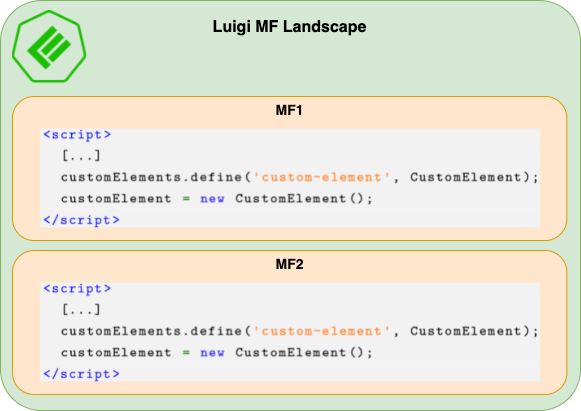
\includegraphics[width=0.6\textwidth]{Figures/customElements_registered.drawio.png}
	\caption{Simple micro frontend landscape using Web Components}
	\label{fig:same_wc_example}
\end{figure}

Figure \ref{fig:same_wc_example} shows a simple micro frontend landscape with Luigi using Web Components. As it is visible, both micro frontends are registering the same tag name \texttt{custom-element} using the \texttt{customElements} object. This object is a read-only property of the \texttt{Window} interface.
The above shown scenario will cause a  \texttt{DOMException}, this way making it impossible to register the same tag twice.

The registration of Web Components follows the \textit{"first come, first served"} principle, the first micro frontend to register a tag name defines this tag and can not be overwritten without reloading the page.\cite{mdn_web_docs_define}

\subsection{Objections}

There is still a niche case which can be raised as an objection. What if even though the tag name is the same, the elements themselves are different? This is a justified objection to the example above. And a conclusion is, that it it is up to the developers to use the standard properly.

Assuming a common micro frontend landscape where every micro frontend is developed by independent, isolated teams, using heterogenic frameworks, the mentioned issue might occur. Two teams use Web Components and try to register different elements under the same tag name in the same landscape. This requires organizational interference on team level.

One way would be to define a name space for every team when creating Web Components e.g. Team 1 has the name space \texttt{team-1}. Making a Web Component registered by the micro frontend of Team 1, be named \texttt{team-1-tagname}. That again could lead to redundancies, because there is no way of assuring that the \texttt{team-1-tagname} and \texttt{team-2-tagname} Web Components are not the same.\cite{wc_best_practices}

A better way might be to assign a common Web Components library like \textbf{UI5 Web Components}. That way the registered elements are provided by the library and are limited to set of unique registrable tags. If another micro frontend would use an already registered element of the library, a warning is thrown but no error occurs.

Most Web Component libraries also offer so called scoping options. This feature finds its use case, when versions of the used components differ from micro frontend to micro frontend. This option enables the developers to customize their Web Components and register them under different tags. That of course might lead to redundancies again. But it also reduces the dependency of the developer teams to always use the latest version of the component library or the first registered element in the landscape. \cite{ui5_webcomponents_scoping} \cite{openwc_scoping}

\section{Webpack Module Federation}
\label{wmf_chap_2}

A rather new way of creating micro frontends is the \textbf{Webpack 5 Module Federation (WMF)}. With the release of version 5 in October 10 in 2020, this technology added certain features which improved its usage for developing micro frontends.\cite{wmf_concepts}

Since the main focus of this document is to propose methods of avoiding redundancies in micro frontend landscapes, an introduction of this WMF feature is given here.

The basic concept of the new WMF involves so called \texttt{hosts} and \texttt{remotes}. These terms are comparable to the \textbf{Luigi Core} and \textbf{Luigi Nodes} principle, previously introduced in section \ref{mf_framework_luigi}. In case of WMF the \texttt{host} aka \texttt{shell} represents the \textbf{Core} or basis of the micro frontend landscape and the \texttt{remotes} or \texttt{micro frontends} are the \textbf{Nodes} integrated or loaded into it. 
Still a direct comparison is not entirely possible since both frameworks look similar functionality-wise, but in their cores work differently. For instance, when using WMF one is tied to use the Webpack bundler, since the necessary configuration is done in the \texttt{webpack.config.js}. This restriction is applied to every micro frontend in the WMF micro frontend landscape, not only to the \texttt{host}.

WMF can be used in combination with most of the common UI Frameworks. But since the implementation for this thesis was done with Angular, the further examples and explanations will be Angular-based.

As explained WMF is a micro frontend framework, but for the purpose of solving the issue introduced in this transcript, it provides functionality too.
This feature is enabled and configured, as well as the rest of the WMF, via the \texttt{webpack.config.js}. When configuring the components of the landscape, it is possible to define a section where shared dependencies are described. These dependencies can be defined in different ways. For instance, it is possible to define a strict version of the dependency, which would result in the framework loading this specific version. Or one can define a less restricted dependency which would mean, that if another \texttt{remote} loads the same dependency but in a different version, the framework would automatically apply the highest major version of the dependency to both micro frontends.
\newpage
\begin{lstlisting}[language=JavaScript, caption=Example of sharing dependencies configured in the \texttt{webpack.config.js}, label=shared_mapping_wmf]
	  shared: share({
			"@angular/core": { 
				singleton: true, 
				strictVersion: false, 
				requiredVersion: '12.2.0' 
			},
			"@angular/common": { 
				singleton: true, 
				strictVersion: false, 
				requiredVersion: '12.2.0' 
			},
			"@fundamental-ngx/core": { 
				singleton: true, 
				strictVersion: false, 
				requiredVersion: '0.33.0-rc.214' 
			},
			
			...sharedMappings.getDescriptors()
		})
\end{lstlisting}

The listing \ref{shared_mapping_wmf} is an example of how to share libraries in a restrictive way. To provide a less restricted configuration a simple array of the shared dependency names suffices. But to ensure a redundant free landscape, these restrictions are necessary. Each configuration property will be explained below.

\begin{itemize}
	\item \texttt{singleton} - This property defines if the dependency should be able to be loaded more than once in different versions or not. If set to \texttt{true}, WMF will automatically pick the highest version of a major release of this dependency available and distribute it to the \texttt{remotes}.\cite{wmf_version_mismatch}
	
	\item \texttt{strictVersion} - This property defines if the dependency requires a specific version to work. If set to \texttt{true} WMF, will load the required version even if another dependency mapping with the same name is present. This can lead to conflicts with the \texttt{singleton} property, if configured poorly.
	
	\item \texttt{requiredVersion} - This property defines the required version of the dependency. When working with a package manager (e.g. NPM), this version has to be aligned with the locally installed version of the dependency. If the \texttt{strictVersion} property is set to \texttt{false}, this property defines the minimum version for the micro frontend. 
	
	It has to be mentioned that, WMF is able to distinguish between major releases. If a higher version of the same major release is available it will be loaded (e.g. \texttt{@angular/common@12.3.1}). For instance, if the next higher version is of a different major release e.g. 13.X.X, WMF would not consider to load it for the \texttt{remotes} which have the \texttt{requiredVersion} of release 12.X.X configured.
\end{itemize}

Now when it comes to sharing the dependencies of inside the micro frontend landscape, each \texttt{remote} has to bulk in. That means each micro frontend has to define its required dependencies in their respective versions. Additionally it has to be mentioned that the micro frontends themselves have to use dynamic imports when importing shared dependencies. Through the asynchronous behavior of the import, Webpack has time to pick the correct version of the dependency inside the landscape.\cite{wmf_concepts}
Analyzing this statement in combination with the information in the above list, it becomes obvious that multiple versions of the same framework can exist in a landscape. The below figure explains it in a graphical way.

\begin{figure}[!h]
	\centering
	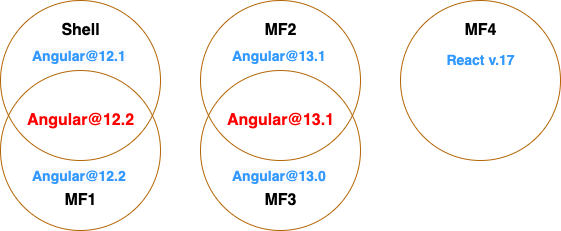
\includegraphics[width=0.7\textwidth]{Figures/multi_version_diagramm.drawio.png}
	\caption{WMF way of handling multi-versions}
	\label{fig:wmf_multiversions}
\end{figure}

As it can be seen in \ref{fig:wmf_multiversions} WMF always picks the the highest major release, assuming the respective micro frontends have the above shown configuration \ref{shared_mapping_wmf} applied. If for instance, if \textbf{MF3} has its \texttt{strictVersion} property set to \texttt{true}, it would cause the loading of its libraries too.

When now looking at the introduced example, it is obvious that sharing several versions of the same framework over the whole landscape can not go without side effects. One of which is the increase in bundle sizes, since every \texttt{remote} bundles their local dependencies. WMF then picks the one to serve during the runtime of the landscape.
This impact has a trade-off tough. Returning users can benefit from cached dependencies but in certain use cases this is not acceptable.\cite{wmf_multi_versions}
 
